%!TEX root = main.tex

\section{Background}
Breast cancer is the number one most common cancer amongst women in Singapore. Early and accurate diagnosis of breast cancer is important for breast-saving and life-saving treatment. \\

The gold standard for the diagnosis of breast cancer is by surgically removing the breast lump with a complete microscopic examination of the breast tissue to look for cancer cells. \\

Fine needle aspiration is an alternative that allows the doctor to take out a small amount of tissue from the breast lump, without the need for surgery to remove the entire breast lump. By examining the characteristics of the cells, doctors have been able to diagnose breast cancer with variable success. Increasing the success of fine needle aspiration allows for diagnosis of breast cancer without the need for a woman to undergo surgery to remove the breast lump. \\

To resolve this, this project uses a fuzzy decision tree to classify breast tumor cells into malignant cancer cells or benign non-cancerous cells. \\

\section{Dataset}
The dataset used was the Breast Cancer Wisconsin (Diagnostic) Data Set from the University of Irvine (UCI) Machine Learning Repository. The dataset contained 569 instances, with no missing data. 357 instances were benign (not cancerous) and 212 were malignant (cancerous). \\

The features were computed from digitalized images of fine needle aspirates of breast tumors. They describe 10 characteristics of the cell nuclei present in the images:

\begin{itemize}
	\item The radius of an individual nucleus
	\item The nuclear perimeter
	\item The nuclear area
	\item Compactness of the nucleus
	\item The smoothness of the contour of the nucleus
	\item The number of contour concavities
	\item The symmetry of the nuclear contour
	\item The texture of the cell nucleus
\end{itemize}

\begin{figure}[h!]
	\centering
	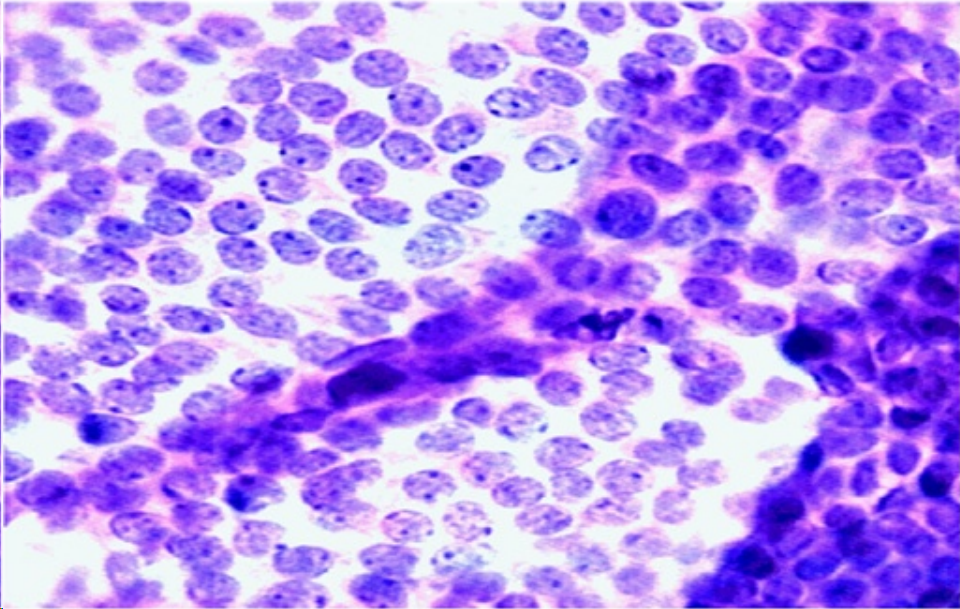
\includegraphics[width=0.4\linewidth]{screenshot001}
	\hspace{0.5cm}
	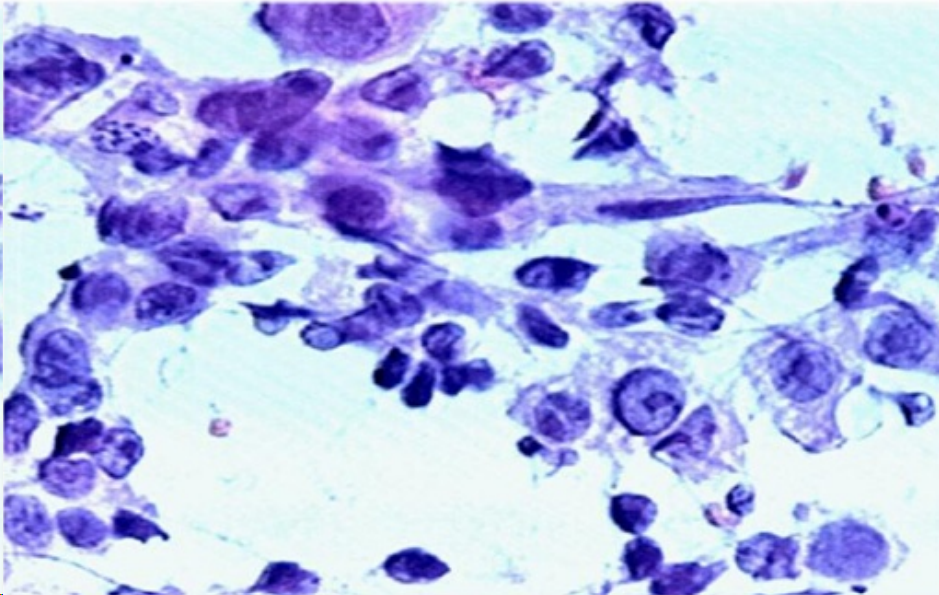
\includegraphics[width=0.4\linewidth]{screenshot002}
	\caption{A picture of breast cells. The cells on the left are begin while the cells on the right are cancerous.}
	\label{fig:images}
\end{figure}

\newpage

The mean, standard error and worst (mean of the three largest values) of these features are computed for each image, resulting in 30 features in the UCI dataset. \\

We follow in the footsteps of Sizilio et al. \ref{fna} and add newly generated features of homogeneity and uniformity that were demonstrated to have diagnostic importance. \\

Uniformity is the difference between the radius worst value and the radius mean value and is an indication of the variability in size of the cell nuclei. \\

Homogeneity is the difference between the worst value of symmetry and the mean value of symmetry and is an indication of the symmetry of the cell nuclei. \\

According to Sizilio et al., the features of area, perimeter, homogeneity and uniformity produced the best results. Thus, we use these 4 feature and drop all other features. \\

\iffalse
The minimum and maximum area, perimeter, homogeneity and uniformity for the 2 labels (benign and malignant) are computed and displayed in the table below. \\

Fuzzy intervals are present for each of the above 4 features, whereby the benign values are within the range of the malignant values. This means that it is not linearly possible to diagnosis a breast lump as benign or malignant using a simple decision tree. Thus, we shall resort to using a fuzzy decision tree. \\

\section{Fuzzy Decision Tree}
A typical decision tree works by building a set of if statements to determine which class something belongs to. \\

At each branch of the decision tree, depending on whether a given statement is true / false, either the left or right path is chosen. \\

On the other hand, a fuzzy decision tree makes use of fuzzy logic, where the truth value of variables can range between 0 and 1 instead of being exactly 0 or exactly 1. \\
\fi

\section{Decision Tree}
To solve this problem, we will make use of a decision tree. \\

\begin{figure}[h!]
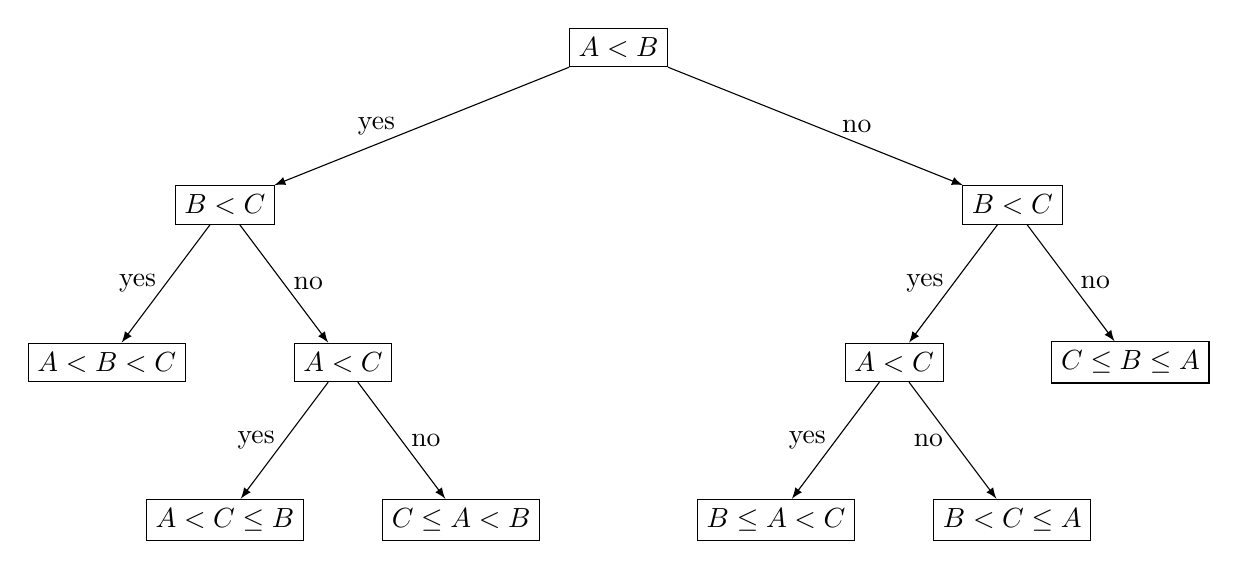
\begin{tikzpicture}[edge from parent/.style={draw,-latex},
level distance=2cm,
level 1/.style={sibling distance=10cm},
level 2/.style={sibling distance=3cm}]
\tikzstyle{every node}=[rectangle,draw]    
\node (Root) {$A < B$}
child {
    node {$B < C$}    
    child { 
        node {$A < B < C$} 
        edge from parent node[left,draw=none] {yes}
    }
    child { 
        node {$A < C$} 
        child {
            node {$A < C \leq B$}
            edge from parent node[left,draw=none] {yes}
        }
        child {
            node {$C \leq A < B$}
            edge from parent node[right,draw=none] {no}
        }
        edge from parent node[right,draw=none] {no}
    }
    edge from parent node[left,draw=none] {yes $\;$}
}
child {
    node {$B < C$}
    child { 
        node {$A < C$}     
        child {
            node {$B \leq A < C$}
            edge from parent node[left,draw=none] {yes}
        }   
        child {
            node {$B < C \leq A$}
            edge from parent node[left,draw=none] {no}
        }     
        edge from parent node[left,draw=none] {yes}
    }
    child { 
        node {$C \leq B \leq A$} 
        edge from parent node[right,draw=none] {no}
    }
    edge from parent node[right,draw=none] { $\;$ no}
};
\end{tikzpicture}
\caption{A decision tree for sorting three values.}
\label{fig:sortingtree}
\end{figure}


\heading{Entropy} A decision tree essentially asks certain questions at the right times, in order to determine which class the input belongs to. To do this, a value known as the entropy with the following formula is used.

$$E = \sum_{i=1}^{C}p_i\log_2 p_i$$

It measures the "impurity" of a set of objects. When the set is homogeneous (i.e. all the objects are of the same class), the entropy will be low. When the set is heterogeneous (i.e. the objects are from different classes), the entropy will be high. \\

\heading{Information Gain} In order to decide what question to ask at which point in time, we need to determine which question results in the greatest decrease in entropy. This is calculated using the information gain shown below:

$$IG = 1 - E$$

The feature that results in the greatest information gain will be selected for that branch of the tree. For continuous features, a threshold will be chosen based on what threshold will result in the greatest information gain. \\

Finally, we need to explain when the decision tree will decide when it should stop splitting. It will do this when a maximum depth $d$ has been reached or when there a fewer than $s$ samples remaining to split. \\

\heading{Pseudocode} With this, we can now construct our decision tree. The pseudocode for construction and inference can be found \ref{fig:pseudocode}.
\begin{itemize}
	\item \textbf{S} is the training data with $m$ classes and $n$ continuous features. It is a set and all \textbf{S} are within $\{\textbf{S} : \textbf{S} = {((f_1,\dots,f_n),c),f_i\in\mathbb{R},c\in [1,m]}\}$
	\item $d$ is the maximum depth that the tree can reach and $s$ the minimum size of the data before we stop branching the tree.
	\item We also define the node object $\textbf{N}$. It has a children attribute $N.\sf{children}$ which is a list of $\eta$ child nodes. $\{\textbf{N}_1,\dots,\textbf{N}_\eta\}$. Furthermore, it also stores a function $\textbf{N}.\sf{func}(\mathnormal{(f_1,f_2,\dots,f_n)})$ which takes in a list of features and outputs an integer $i\in[1,\eta]$. The depth of the node in the tree is also stored in $\textbf{N}.\sf{depth}$
\end{itemize}


\begin{figure}[h]
	\oneCol{.9}{
		\alg{$\sf{CalculateEntropy}(\bf{S}, t)$}
		$I\gets0$\\
		$\textbf{S}_1\gets\{((f_1,\dots,f_n),c) : f_i<t, ((f_1,\dots,f_n),c)\in \textbf{S}\}$\\
		$\textbf{S}_2\gets\{((f_1,\dots,f_n),c) : f_i>t, ((f_1,\dots,f_n),c)\in \textbf{S}\}$\\
		$\textbf{C}_1\gets\{c : ((f_1,\dots,f_n),c)\in \textbf{S}_1\}$\\
		$\textbf{C}_2\gets\{c : ((f_1,\dots,f_n),c)\in \textbf{S}_2\}$\\
		$I\gets1-\frac{|\textbf{C}_1|\times E(\textbf{C}_1)+|\textbf{C}_2|\times E(\textbf{C}_2)}{|\textbf{S}|}$\\
		Return $\textbf{S}_1,\textbf{S}_2,I$\\
		
		\alg{$\sf{BuildTree}(\bf{S}, \mathnormal{d, s})$}
		Initialise new node $\textbf{N}$\\
		Initialise empty queue $\bf{L}$\\
		$\textbf{N}_{root}\gets\textbf{N}$\\
		$\textbf{L}.\sf{push}((\textbf{S},\textbf{N}))$\\
		While $\textbf{L}.\sf{size}\neq0$ do\\
		\ind $\textbf{S}, \textbf{N}\gets \textbf{L}.\sf{pop}()$ \\
		\ind If $\textbf{N}.\sf{depth} > \mathnormal{d}$ or $|\textbf{S}|<s$ then break \\
		\ind $I_{max}\gets0$ \\
		\ind For $i\in1\dots n$ do \\
		\ind \ind $E\gets 0$ \\
		\ind \ind For $t\in \{f_i : ((f_1,\dots,f_n),c)\in \textbf{S}\}$ do \\
		%\ind \ind \ind $\textbf{S}_{less}\gets\{((f_1,f_2,\dots,f_n),c) : f_i<t, ((f_1,f_2,\dots,f_n),c)\in \textbf{S}\}$ \\
		%\ind \ind \ind $\textbf{S}_{more}\gets\{((f_1,f_2,\dots,f_n),c) : f_i>t, ((f_1,f_2,\dots,f_n),c)\in \textbf{S}\}$ \\
		\ind \ind \ind $\textbf{S}_1,\textbf{S}_2,I\gets\sf{CalculateEntropy}\mathnormal{(\textbf{S}, t)}$ \\
		\ind \ind \ind If $I_{max} < I$ then \\
		\ind \ind \ind \ind $I_{max}\gets I; i_{max}\gets i; t_{max}\gets t$ \\
		\ind \ind \ind \ind $\textbf{S}_3\gets \textbf{S}_1; \textbf{S}_4\gets \textbf{S}_2$ \\
		\ind \ind \color{gray}{End if} \\
		\ind \color{gray}{End for} \\
		\color{black}
		\ind Initialise new nodes $\textbf{M}_l, \textbf{M}_r$ \\
		\ind $\textbf{M}_l.\sf{\textbf{p}}=\mathnormal{\frac{|\{c : c == 1,((f_1,\dots,f_n),c)\in \textbf{S}_1\}|}{|\textbf{S}_1|}}$\\
		\ind $\textbf{M}_r.\sf{\textbf{p}}=\mathnormal{\frac{|\{c : c == 1,((f_1,\dots,f_n),c)\in \textbf{S}_2\}|}{|\textbf{S}_2|}}$\\
		\ind $\textbf{N}.\sf{func}\gets\mathnormal{((f_1,\dots,f_n)}\mapsto \sf{If}\;\mathnormal{f_{i_{max}}<t_{max}}\;0\;\sf{then}\;1)$\\
		\ind $\textbf{N}.\sf{children}[0]\gets\mathnormal{\textbf{M}_l}$ \\
		\ind $\textbf{N}.\sf{children}[1]\gets\mathnormal{\textbf{M}_r}$ \\
		\ind $\textbf{L}.\sf{push}\mathnormal{((\textbf{S}_3,\textbf{M}_l))}$\\
		\ind $\textbf{L}.\sf{push}\mathnormal{((\textbf{S}_4,\textbf{M}_r))}$\\
		\ind \color{gray}{End for} \\
		\color{gray}{End while}\\
		\color{black}Return $\textbf{N}_{root}$\\ \\
		
		\alg{$\sf{Qry({f_1,\dots,f_n},\textbf{N})}$}
		$i\gets\textbf{N}.\sf{func}({f_1,\dots,f_n})$\\
		If $\textbf{N}.$$\sf{children}$$[i]=\bot$ then\\
		\ind If $\textbf{N}.\textbf{p} < 0.5$ then \\
		\ind \ind Return 0\\
		\ind else return 1\\
		Else \\
		\ind Return $\sf{Qry}$(${f_1,\dots,f_n},\mathnormal{\textbf{N}.\sf{children}[i]}$)\\
	}
	\vspace{-.5cm}
	\caption{Pseudocode for construction and inference of the tree.}
	\label{fig:pseudocode}
	\vspace{-.5cm}
\end{figure}

\heading{Time Complexity} Now, let us analyse the time and space complexity of our algorithm. 
\begin{itemize}
	\item Let us assume that the tree will be fully filled with height $d$. This means that there will be $2^{d+1}-1$ nodes in the tree. This means the split would have been done $2^{d}-1$ times. In practice, this may not be true but let's assume so for the sake of simplicity.
	\item Splitting the tree has a time-complexity of $O(n\times|\textbf{S}|^2)$ where $|\textbf{S}|$ is the length of the data that still remains at that node and $n$ is the number of features. This is because calculating the entropy has time-complexity $O(|\textbf{S}|)$ and there $|\textbf{S}|$ thresholds to compute and $n$ features to compute them for.
	\item Now,let's denote the size of the dataset at depth $x$ and at the $i^{th}$ node as $|\textbf{S}_{x,i}|$. We know that $|\textbf{S}|=\sum_{i=1}^{2^x}|\textbf{S}_{x,i}|$. 
	\item On average, we can assume that $|\textbf{S}|$ will be halved at each split. Thus,
	$$|\textbf{S}_{x,i}|=\frac{|\textbf{S}|}{2^x}$$
	\item Then, the total average time-complexity for training the decision tree is 
	$$O(\sum_{x=0}^{d}\sum_{i=1}^{2^x}n\times|\textbf{S}_{x,i}|^2)=O(\sum_{x=0}^{d}n\times\frac{|\textbf{S}|^2}{2^x})=O(n\times|\textbf{S}|^2\times(2-2^{-d}))=O(n\times|\textbf{S}|^2)$$
	\item In the worst case, let's say that the dataset is split unevenly such that all the sample except one go to the next node. Then, $|\textbf{S}_{x,0}|=|\textbf{S}|-x$ and $|\textbf{S}_{x,1}|=1$.
	\item Then, the total worst-case time-complexity for training the decision tree is
	$$O(\sum_{x=0}^{d}\sum_{i=1}^{2^x}n\times|\textbf{S}_{x,i}|^2)=O(\sum_{x=0}^{d}n\times(|\textbf{S}|^2+1))=O(n\times d\times|\textbf{S}|^2)$$
	\item Now, let's calculate the memory complexity of training the tree. Calculating the entropy requires creating the new dataset splits to be handed to the children nodes. This is done in $O(|\textbf{S}_{x,i}|)$ space because the size of 2 new dataset splits must add up to the dataset they were split from. For simplicity, let's assume none of this memory is deallocated. Then, the memory complexity is 
	$$O(\sum_{x=0}^{d}\sum_{i=1}^{2^x}|\textbf{S}_{x,i}|)=O(d\times|\textbf{S}|)$$
	\item Now, let's calculate the time complexity of inference. Deciding which path to take in a decision tree is O(1). Thus, for a tree of height $d$ and average height $\bar{d}$, the worst-case time-complexity is $O(d)$ and $O(\bar{d})$. The memory complexity is $O(1)$ because no additional space is needed during inference other than the space needed to store the tree.
\end{itemize}

\section{Random Forest}
To improve the performance of our classifier, we make use of many different decision tree classifiers in an ensemble.



\tikzset{
  font=\Large\sffamily\bfseries,
  red arrow/.style={
    midway,red,sloped,fill, minimum height=3cm, single arrow, single arrow head extend=.5cm, single arrow head indent=.25cm,xscale=0.3,yscale=0.15,
    allow upside down
  },
  black arrow/.style 2 args={-stealth, shorten >=#1, shorten <=#2},
  black arrow/.default={1mm}{1mm},
  tree box/.style={draw, rounded corners, inner sep=0.5em},
  node box/.style={white, draw=black, text=black, rectangle, rounded corners},
}


\begin{centering}
\begin{forest}
  for tree={l sep=1.3em, s sep=1.3em, anchor=center, inner sep=0.5em, fill=blue!50, circle, where level=2{no edge}{}}
  [
  Training Data, node box
  [sample and feature bagging, node box, alias=bagging, above=3em
  [,red!70,alias=a1[[,alias=a2][]][,red!70,edge label={node[above=1ex,red arrow]{}}[[][]][,red!70,edge label={node[above=1ex,red arrow]{}}[,red!70,edge label={node[below=1ex,red arrow]{}}][,alias=a3]]]]
  [,red!70,alias=b1[,red!70,edge label={node[below=1ex,red arrow]{}}[[,alias=b2][]][,red!70,edge label={node[above=1ex,red arrow]{}}]][[][[][,alias=b3]]]]
  [~~$\dots$~,scale=2,no edge,fill=none,yshift=-4em]
  [,red!70,alias=c1[[,alias=c2][]][,red!70,edge label={node[above=1ex,red arrow]{}}[,red!70,edge label={node[above=1ex,red arrow]{}}[,alias=c3][,red!70,edge label={node[above=1ex,red arrow]{}}]][,alias=c4]]]]
  ]
  \node[tree box, fit=(a1)(a2)(a3)](t1){};
  \node[tree box, fit=(b1)(b2)(b3)](t2){};
  \node[tree box, fit=(c1)(c2)(c3)(c4)](tn){};
  \node[below right=0.3em, inner sep=0pt] at (t1.north west) {Tree 1};
  \node[below right=0.3em, inner sep=0pt] at (t2.north west) {Tree 2};
  \node[below right=0.3em, inner sep=0pt] at (tn.north west) {Tree $n$};
  \path (t1.south west)--(tn.south east) node[midway,below=4em, node box] (mean) {mean in regression or majority vote in classification};
  \node[below=1em of mean, node box] (pred) {prediction};
  \draw[black arrow={5mm}{4mm}] (bagging) -- (t1.north);
  \draw[black arrow] (bagging) -- (t2.north);
  \draw[black arrow={5mm}{4mm}] (bagging) -- (tn.north);
  \draw[black arrow={5mm}{5mm}] (t1.south) -- (mean);
  \draw[black arrow] (t2.south) -- (mean);
  \draw[black arrow={5mm}{5mm}] (tn.south) -- (mean);
  \draw[black arrow] (mean) -- (pred);
\end{forest}
\end{centering}


In essence, the data is split into multiple non-overlapping parts. A decision tree is trained on each part and together they form an ensemble. To obtain the final prediction, majority voting is used on the outputs of each decision tree. If more decision trees predict that the cells are benign, the prediction of the random forest will be benign. On the other hand, if more decision trees predict that the cells are malignant, the output of the random forest will be that the cells are malignant. \\

\heading{Time Complexity} The time complexity for the Random Forest Classifier is similar to that of the standard Decision Tree as the Decision Tree underpins the structure of the Random Forest Classifier.
\begin{itemize}
	\item Let us assume that the tree will be fully filled with height $d$. This means that there will be $2^{d+1}-1$ nodes in the tree. This means the split would have been done $2^{d}-1$ times. In practice, this may not be true but let's assume so for the sake of simplicity.
	\item Splitting the tree has a time-complexity of $O(n\times|\textbf{S}|^2)$ where $|\textbf{S}|$ is the length of the data that still remains at that node and $n$ is the number of features. This is because calculating the entropy has time-complexity $O(|\textbf{S}|)$ and there $|\textbf{S}|$ thresholds to compute and $n$ features to compute them for.
	\item Now,let's denote the size of the dataset at depth $x$ and at the $i^{th}$ node as $|\textbf{S}_{x,i}|$. We know that $|\textbf{S}|=\sum_{i=1}^{2^x}|\textbf{S}_{x,i}|$. 
	\item On average, we can assume that $|\textbf{S}|$ will be halved at each split. Thus,
	$$|\textbf{S}_{x,i}|=\frac{|\textbf{S}|}{2^x}$$
	\item Then, the total average time-complexity for training the decision tree is 
	$$O(\sum_{x=0}^{d}\sum_{i=1}^{2^x}n\times|\textbf{S}_{x,i}|^2)=O(\sum_{x=0}^{d}n\times\frac{|\textbf{S}|^2}{2^x})=O(n\times|\textbf{S}|^2\times(2-2^{-d}))=O(n\times|\textbf{S}|^2)$$
	\item In the worst case, let's say that the dataset is split unevenly such that all the sample except one go to the next node. Then, $|\textbf{S}_{x,0}|=|\textbf{S}|-x$ and $|\textbf{S}_{x,1}|=1$.
	\item Then, the total worst-case time-complexity for training the decision tree is
	$$O(\sum_{x=0}^{d}\sum_{i=1}^{2^x}n\times|\textbf{S}_{x,i}|^2)=O(\sum_{x=0}^{d}n\times(|\textbf{S}|^2+1))=O(n\times d\times|\textbf{S}|^2)$$
	\item Now, let's calculate the memory complexity of training the tree. Calculating the entropy requires creating the new dataset splits to be handed to the children nodes. This is done in $O(|\textbf{S}_{x,i}|)$ space because the size of 2 new dataset splits must add up to the dataset they were split from. For simplicity, let's assume none of this memory is deallocated. Then, the memory complexity is 
	$$O(\sum_{x=0}^{d}\sum_{i=1}^{2^x}|\textbf{S}_{x,i}|)=O(d\times|\textbf{S}|)$$
	\item Now, let's calculate the time complexity of inference. Deciding which path to take in a decision tree is O(1). Thus, for a tree of height $d$ and average height $\bar{d}$, the worst-case time-complexity is $O(d)$ and $O(\bar{d})$. The memory complexity is $O(1)$ because no additional space is needed during inference other than the space needed to store the tree.
\end{itemize}

\section{Performance}

Now, we shall evaluate the performance of our model. The results are summarised in the table below.

\section{GUI}


\section{Reflections}
\heading{Matthew} Coding the decision tree from scratch was enjoyable and it allowed me to have an under the hood understanding of an important machine learning algorithm. An improvement that we could have made as a group was to do more planning in the beginning. We had to reverse some decisions to improve on our final product. Despite this, my group worked very well together as a team as we are good friends to begin with (and somehow managed to be in the same team even though it was RNG). Overall, I have always liked data structures and algorithms and this module was both educational and enjoyable.

\heading{Jed} I was largely responsible for writing the report and coding out the GUI. From writing the report, I learnt alot about about writing good and clear pseudocode as well as writing good mathematical analysis on time-complexity and space-complexity. For the GUI, instead of using JavaFX, I made use of Jetpack Compose for Desktop. It was much easier to use and it has replaced JavaFX in many projects that I am doing. Overall, I enjoyed working on this task but I found the need for the tree to used for a social cause very restricting. The task would be easier and much more fun if we have the flexibility of using a tree for whatever purpose we want such as quad-trees / oct-trees for gravitational simulations. Also having more flexibility in what language we can use for the assignment and the module in general would be nice because data structures and algorithms can be implemented in any language, not just Java.

\heading{Zayan} This project was interesting and challenging. At first, I was tasked to code out the decision tree with the algorithm ID3 (Iterative Dichromatizer 3) with binning. This was challenging to code as it involved a lot of resizing. However, all my work was scrapped because we decided to pivot and used a different decision tree algorithm which Matthew coded out. It was tough seeing your work thrown out but it was a necessary part to put out the best work. I learnt that sometimes in life you have to make tough decisions and redo stuff for the best result. I then coded out the random forest classifier and the metric algorithms and also helped refactor some of the decision tree code. All in all, it was a fun experience.

\heading{Mayukh}
